%%%%%%%%%%%%%%%%%%%%%%%%%%%%%%%%%%%%%%%%%
% University/School Laboratory Report
% LaTeX Template
% Version 3.1 (25/3/14)
%
% This template has been downloaded from:
% http://www.LaTeXTemplates.com
%
% Original author:
% Linux and Unix Users Group at Virginia Tech Wiki 
% (https://vtluug.org/wiki/Example_LaTeX_chem_lab_report)
%
% License:
% CC BY-NC-SA 3.0 (http://creativecommons.org/licenses/by-nc-sa/3.0/)
%
%%%%%%%%%%%%%%%%%%%%%%%%%%%%%%%%%%%%%%%%%

%----------------------------------------------------------------------------------------
%	PACKAGES AND DOCUMENT CONFIGURATIONS
%----------------------------------------------------------------------------------------

\documentclass{article}

\usepackage[version=3]{mhchem} % Package for chemical equation typesetting
\usepackage{siunitx} % Provides the \SI{}{} and \si{} command for typesetting SI units
\usepackage{graphicx} % Required for the inclusion of images
\usepackage{natbib} % Required to change bibliography style to APA
\usepackage{amsmath} % Required for some math elements 
\usepackage[boxed]{algorithm2e} % required for algorithms
\usepackage{fancyhdr}

%\setlength\parindent{0pt} % Removes all indentation from paragraphs; ignore this

\renewcommand{\labelenumi}{\alph{enumi}.} % Make numbering in the enumerate environment by letter rather than number (e.g. section 6)

\pagestyle{fancy}
\fancyhf{}
\lhead{Whitacre School of Engineering}
\rhead{Texas Tech University}
\rfoot{\thepage}
\lfoot{TR 2015-001}

%\usepackage{times} % Uncomment to use the Times New Roman font

%----------------------------------------------------------------------------------------
%	DOCUMENT INFORMATION
%----------------------------------------------------------------------------------------

\title{GoblinCore64: \\ Architectural Specification \\ Technical Report 2015-001} % Title

\author{John D. \textsc{Leidel}} % Author name

\date{\today} % Date for the report

\begin{document}

\maketitle % Insert the title, author and date

\begin{center}
\begin{tabular}{l r}
Version: & 1.0 \\ % Date the experiment was performed
Texas Tech University \\ % Partner names
Data Intensive Scalable Computing Laboratory \\ % Course

\end{tabular}
\end{center}

\newpage

\tableofcontents

\newpage

%----------------------------------------------------------------------------------------
%	SECTION 1
%----------------------------------------------------------------------------------------
\section{Introduction}

\subsection{GC64 Overview}

The GoblinCore-64 (herein referred to as GC64) that was originally designed to 
facilitate the construction of a high performance core architecture that was
well-suited to executing applications traditionally known as "data intensive."  
These applications generally refer to algorithms that operate on sparse
data structures such as graphs, sparse matrices and/or perform nonlinear 
combinatorial operations (et.al.).  We consider all of the aforementioned target
application areas to share the following two general characteristics.  

\begin{itemize}
\item \textbf{Non-Unit Stride}: All of the applications we consider as design targets
for GC64 perform a disproportionate number of non-unit stride computations.  These 
  computations may simply be non-unit stride, scatters, gathers or completely random. 
  In all cases, the data elements are not generally well-suited to traditional 
  long SIMD or data caching architectures.
\item  \textbf{Memory Intensive}: Given the first characteristic, we also assume
  a latent characteristic with respect to the memory bandwidth requirements.  
  Given the sparsity or non-linear access requirements, we assume that the design 
  targets operate with a disproportionally high bandwidth to compute ratio.  As
  such, we consider them to be memory intensive rather than computationally
  intensive.  
\end{itemize} 

In addition to the core design requirements, we also sought to build a
completely open source architecture and tool chain suitable for architectural 
research in academia and possible commercial implementations.  As such, we sought
to build BSD-like licensing around the core ISA, simulation infrastructure, tools
and toolchain.  Given this, we found that our implementation goals aligned 
well with the RISC-V project \cite{Waterman:EECS-2014-54}.  These include, but are
not limited to the following: 

\begin{itemize}
\item A completely \emph{open} ISA that is freely available to academia and industry.
\item An ISA separated into a \emph{small} base integer ISA. 
\item Support for the revised 2008 IEEE-754 \cite{2008IEEE} floating-point standard.
\item An ISA with \emph{native} support for highly-parallel multicore or many core
implementations.  
\end{itemize}

In addition to the core RISC-V goals, we also wanted to achieve the following
architectural goals (as related to our target design requirements): 

\begin{itemize}
\item Provide simple architectural structures that are conducive to constructing
  highly (MIMD) parallel and concurrent applications
\item Provide simple ISA extensions conducive to compiler optimization of
concurrent applications
\item Provide a low-level, mutable parallel construct in hardware that can
  be easily mapped to higher level parallel programming models (threads, tasks, etc)
\item Provide hardware mechanisms to minimize context switch latency to a very small
  number of cycles (goal of single cycle context switching events)
\item Provide a well-defined mechanism when context switch events occur
\item Provide a well-defined mechanism for user applications to explicitly induce
  context switch events
\end{itemize}

\subsection{RISC-V ISA Requirements}

The GC64 RISC-V extension functions as both a core RISC-V \cite{Waterman:EECS-2014-54} architectural extension and an extension to the standard 64-bit RISC-V IMAFD specification.  The following minimum architectural extensions are required to utilize GC64.  

\begin{itemize}
\item \textbf{RV64I}:  GC64 requires 64-bit addressing at minimum.  The RV32I memory model is supported as a result.  However, given the use of HMC devices, we require the use of at least 64-bit addressing (and addressing arithmetic).  
\item \textbf{M-Extension}:  GC64 requires the integer multiplication and division for the purpose of efficiently performing address manipulation.  
\item \textbf{A-Extension}: GC64 requires the atomic instructions.
\end{itemize}

The following architectural extensions are supported in the GC64 tasking model.  They are herein named as optional extensions.  

\begin{itemize}
\item \textbf{F-Extension}:  By default, the GC64 task context definition supports the storage of the single precision floating point register values.  If the F-extension is not present, these values are ignored.  
\item \textbf{D-Extension}: By default, the GC64 task context definition supports the storage of the double precision floating point register values.  If the D-extension is not present, these values are ignored.  
\item \textbf{RV128I}: By default, the GC64 reuqires 64-bit addressing.  However, when building scalable versions of GC64 in large SMP or PGAS modes, it may be desirable to support 128bit addressing.  
\end{itemize}

%--- GC64 SoC Architecture
\subsection{GC64 SoC Architecture}

%------ Overview
\subsubsection{Overview}

The GC64 SoC architecture consists of six hierarchical units that
are explicitly organized to provide high degrees of local and global
concurrency without sacrificing performance.  The hierarchy of
architectural units organized from smallest (least encompassing)
to the largest (most encompassing) is depicted in the table below.
Note that each subsequent layer encompasses one or more units from
the previous layer.  At least one of the lower four architectural
layers must be included in all GC64 configurations.

\begin{center}
\begin{itemize}
\item Task Unit [required]
\item Task Processor [required]
\item Task Group [required]
\item Socket [required]
\item Node [optional]
\item Partition [optional]
\end{itemize}
\end{center}

%------ Task Unit
\subsubsection{Task Unit}

The GC64 \emph{Task Unit} is the smallest unit of divisible concurrency.  
The task unit consists of the  RISC-V integer register file, the RISC-V
floating-point register file, the GC64 user-visible registers and the GC64
machine state registers.  

\begin{figure}[h!]
\begin{center}
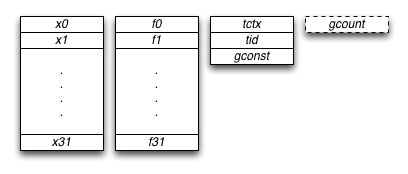
\includegraphics[width=0.75\textwidth]{gc64-task-unit.png}
\caption{GC64 Task Unit}
\end{center}
\label{figure:taskunit}
\end{figure}  

%------ Task Processor
\subsubsection{Task Processor}

The GC64 \emph{Task Processor} consists of the basic integer and floating-point 
arithmetic units, a thread control unit and one or more task units.  The thread control 
unit is essentially an ALU dedicated to managing the state of the task units.  This includes
the following functions: 

\begin{itemize}
\item Spawning new tasks
\item Joining executing tasks
\item Incrementing the task execution pressure [\emph{gcount}]
\item Enforcing context switch events
\end{itemize}

The task processor is permitted to execute instructions from a single task unit on any given 
cycle.  In this manner, each task processor is myopic in its focus.  It is the job of the thread control
unit to enforce which task unit is in \emph{focus} on any given cycle.  Any time the thread control 
unit switches focus from one task unit to an adjacent task unit, we refer to this event as a
\emph{context switch}.  The thread control unit may select a new task unit only 
from the task units that are directly attached.  GC64 requires that at least one task unit
exist per task processor.  GC64 permits a maximum of 256 task units per task processor. 

\begin{figure}[h!]
\begin{center}
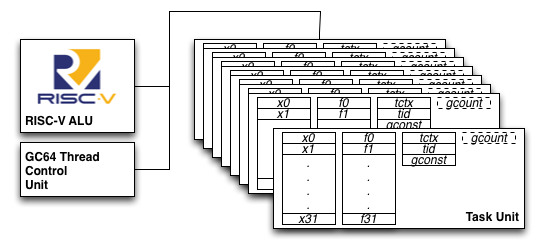
\includegraphics[width=0.75\textwidth]{gc64-task-proc.png}
\caption{GC64 Task Processor}
\end{center}
\label{figure:taskproc}
\end{figure}  


%------ Task Group
\subsubsection{Task Group}

\begin{figure}[h!]
\begin{center}
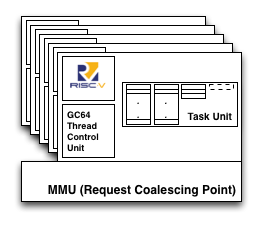
\includegraphics[width=0.75\textwidth]{gc64-task-group.png}
\caption{GC64 Task Group}
\end{center}
\label{figure:taskgroup}
\end{figure}  

%------ Socket
\subsubsection{Socket}

\begin{figure}[h!]
\begin{center}
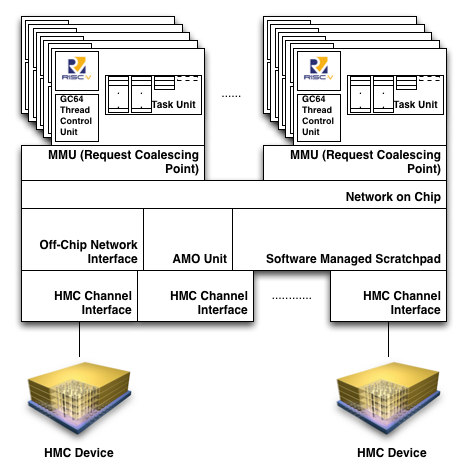
\includegraphics[width=0.75\textwidth]{gc64-socket.png}
\caption{GC64 Socket}
\end{center}
\label{figure:socket}
\end{figure}  

%------ Node
\subsubsection{Node}

%------ Partition
\subsubsection{Partition}

%--- GC64 Memory Organization
\subsection{GC64 Memory Organization}

\subsubsection{Memory Architecture}

\subsubsection{Physical Addressing}

%----------------------------------------------------------------------------------------
%	SECTION 2
%----------------------------------------------------------------------------------------
\section{GC64 Instruction Set Extension}

The GC64 RISC-V instruction set extension can be classified as a \emph{brownfield extension} with respect to the machine state.  In this manner, all the instructions fit within the existing RISC-V encodings.  However, the GC64 extension does instantiate additional machine state in terms of user-visible and non user-visible registers.  

\subsection{GC64 RISC-V Machine Organization}

\subsection{GC64 Register State}
In addition to the registers defined as a part of the base RISC-V IMAFD ISA, we define an additional set of registers for the GC64 extension.  The register extension is defined in terms of User-Visible, Supervisor and Machine-State registers.  User-Visible registers are those that can be read and written from normal user instructions.  Supervisor registers are those that can only be read and written from supervisor-privileged instructions.  Machine-State registers cannot be read or written from any instruction space.  Rather, these registers are implicitly modified during the normal operation of the core.     

\subsubsection{User-Visible Registers} 
The GC64 extension adds a register, \emph{tctx}, to the list of user-visible registers.  The \emph{tctx} register is an unsigned 64bit register that exists per task and contains the base address of the task that is currently loaded in the task unit. The \emph{tctx} register can be read from and written to using user-privileged instructions.  However, given that it resides outside the base RISC-V IMAFD register set, it can only be read from and written to using the \emph{gettask} and \emph{settask} instructions.  

\begin{center}
\makebox[\textwidth][s]{63 0}
\framebox[\textwidth][c]{TCTX}
\end{center}

The GC64 extension adds a task ID register, \emph{tid}, to the list of user-visible registers.  The \emph{tid} register contains an unsigned 64bit value that represents the task ID currently loaded in the respective task unit.  The \emph{tid} registers can be read from a single user-privileged instruction, \emph{gettid}.  

\begin{center}
\makebox[\textwidth][s]{63 0}
\framebox[\textwidth][c]{TID}
\end{center}

The GC64 extension also adds a configuration register, \emph{gconst} that is user-visible.  The \emph{gconst} register is an unsigned 64bit register that contains the configuration parameters for the containing task unit and GC64 processor.  The \emph{gconst} register can only be read.  It cannot be written to.  It can only be read via the \emph{getgconst} instruction.  The \emph{gconst} register contains the following fields.  

\begin{center}
\begin{tabular}{| c | c | c | c |}
\hline
Mnemonic & Bits & Size [Bits] & Description \\ 
\hline \hline
PID & [15:0] & 16 & Partition ID \\
\hline
NID & [31:16] & 16 & Node ID \\
\hline
SID & [39:32] & 8 & Socket ID \\
\hline
TG & [47:40] & 8 & Task Group \\
\hline 
TP & [55:48] & 8 & Task Processors per Task Group \\
\hline 
TC & [63:56] & 8 & Task Units per Task Processor \\
\hline 

\end{tabular}
\end{center} 

\begin{center}
\makebox[\textwidth][s]{63 0}
\framebox[\textwidth][c]{GCONST}
\end{center}

\subsubsection{Supervisor Registers}

The GC64 extension contains a single supervisor register.  This register is contained within each task unit and is referred to as the \emph{gkey} register.  The purpose of this register is to contain the security key loaded via the kernel and constructor routines at application launch such that rogue tasks cannot spawn tasks in the process space of a neighboring process.  Given the purpose of this register, it remains a part of the standard context for context save and restore operations.  This register is represented using as an unsigned 64bit value.  It can be read from and written to using the supervisor instructions \emph{gkey} and \emph{skey}.  

\begin{center}
\makebox[\textwidth][s]{63 0}
\framebox[\textwidth][c]{GKEY}
\end{center}

\subsubsection{Machine-State Registers}

The GC64 extension contains a single machine-state register.  This register, known as the \emph{gcount} register, is not directly readable or writable from any instructions.  Its value is similar in function to a traditional performance counter register.  Any time an instruction is retired through the pipeline, this value is incremented.  The increment value is dependent upon the cost of the retired instruction.  Once this counter reaches its maximum value as defined by the internal architecture state, the encountering task unit is forced to context switch and thus permit another task unit to execute.  The only method the user-privileged code has to indirectly access this register state is the \emph{ctxsw} instruction.  The \emph{ctxsw} instruction explicitly sets this register to its maximum value, thus forcing a context switch event.    

\newpage
\subsubsection{GC64 Register Indexing}
A summary of the permissible GC64 register indices is as follows.
Note that all register follow a 5-bit encoding schema in order to adhere
to the base RISC-V \emph{R-Type} instruction encoding.  
Note that all supervisor registers appear in the index range above 0b10000.

\begin{center}
\begin{tabular}{| l | c | c | }
\hline
Mnemonic & Index & Access \\ \hline
\hline
tctx & 0b00000 & User,Supervisor \\
\hline
tid & 0b00001 & User,Supervisor \\
\hline
gconst & 0b00010 & User,Supervisor \\
\hline
gkey & 0b10000 & Supervisor\\
\hline
\end{tabular}
\end{center}


%------- INTEGER LOAD/STORE INSTRUCTIONS
\subsection{Integer Load/Store Instructions}

The integer load and store instructions require a full 32-bit
instruction encoding space.  We utilize the standard RISC-V
\emph{R-type} ISA encoding format for each of instructions.  In
this manner, all the integer load and store instructions support
three operands and no bundled immediate values.  All explicit index
values for scatter/gather store/load operations must be explicitly
loaded to an integer register (\emph{x0-x31}).

The following load and store instructions share the same base
opcode, but differ in their funct7 field encodings.  The instruction
encoding space is depicted as follows:


\begin{center}
\textbf{GC64 Integer Load Instructions}
\makebox[0.9in][s]{31 25}\makebox[0.03in][s]{}\makebox[0.7in][s]{24 20}\makebox[0.03in][s]{}\makebox[0.6in][s]{19 15}\makebox[0.03in][s]{}\makebox[0.7in][s]{14 12}\makebox[0.03in][s]{}\makebox[0.7in][s]{11 7}\makebox[0.03in][s]{}\makebox[0.9in][s]{6 0}
\framebox[0.9in]{0000000}\framebox[0.7in]{rs2}\framebox[0.7in]{rs1}\framebox[0.7in]{funct3}\framebox[0.7in]{rd}\framebox[0.9in]{0111111}
\end{center}

\begin{center}
\textbf{GC64 Integer Store Instructions}
\makebox[0.9in][s]{31 25}\makebox[0.03in][s]{}\makebox[0.7in][s]{24 20}\makebox[0.03in][s]{}\makebox[0.6in][s]{19 15}\makebox[0.03in][s]{}\makebox[0.7in][s]{14 12}\makebox[0.03in][s]{}\makebox[0.7in][s]{11 7}\makebox[0.03in][s]{}\makebox[0.9in][s]{6 0}
\framebox[0.9in]{0000001}\framebox[0.7in]{rs2}\framebox[0.7in]{rs1}\framebox[0.7in]{funct3}\framebox[0.7in]{rd}\framebox[0.9in]{0111111}
\end{center}



%-- integer gathers
\subsubsection{lbgthr rd, rs1, rs2}

Perform a one-byte \emph{gathered load} operation of the address and
index \emph{rs1} and \emph{rs2}, respectively, and store the result
to the intger register \emph{rd}.  The load portion of the operation
sign extends to the size of the register.  
The operation to perform is as follows:

\begin{equation}
rd = rs1[rs2]
\end{equation}

The effective address to load
from is formed using the following methodology:

\begin{equation}
Effective = addr(rs1 + ((rs2 * 1))
\end{equation}


\subsubsection{lhgthr rd, rs1, rs2}

Perform a two-byte \emph{gathered load} operation of the address and
index \emph{rs1} and \emph{rs2}, respectively, and store the result
to the intger register \emph{rd}.  The load portion of the operation
sign extends to the size of the register.
The operation to perform is as follows:

\begin{equation}
rd = rs1[rs2]
\end{equation}

The effective address to load
from is formed using the following methodology:

\begin{equation}
Effective = addr(rs1 + ((rs2 * 2))
\end{equation}


\subsubsection{lwgthr rd, rs1, rs2}

Perform a four-byte \emph{gathered load} operation of the address and
index \emph{rs1} and \emph{rs2}, respectively, and store the result
to the intger register \emph{rd}.  The load portion of the operation
sign extends to the size of the register.
The operation to perform is as follows:

\begin{equation}
rd = rs1[rs2]
\end{equation}

The effective address to load
from is formed using the following methodology:

\begin{equation}
Effective = addr(rs1 + ((rs2 * 4))
\end{equation}

\subsubsection{ldgthr rd, rs1, rs2}

Perform an eight-byte \emph{gathered load} operation of the address and
index \emph{rs1} and \emph{rs2}, respectively, and store the result
to the intger register \emph{rd}.  The operation to perform is as follows:

\begin{equation}
rd = rs1[rs2]
\end{equation}

The effective address to load
from is formed using the following methodology:

\begin{equation}
Effective = addr(rs1 + ((rs2 * 8))
\end{equation}

\subsubsection{lbugthr rd, rs1, rs2}

Perform a one-byte \emph{gathered load} operation of the address and
index \emph{rs1} and \emph{rs2}, respectively, and store the result
to the intger register \emph{rd}.  The load portion of the operation
zero extends to the size of the register.
The operation to perform is as follows:

\begin{equation}
rd = rs1[rs2]
\end{equation}

The effective address to load
from is formed using the following methodology:

\begin{equation}
Effective = addr(rs1 + ((rs2 * 1))
\end{equation}

\subsubsection{lhugthr rd, rs1, rs2}

Perform a two-byte \emph{gathered load} operation of the address and
index \emph{rs1} and \emph{rs2}, respectively, and store the result
to the intger register \emph{rd}.  The load portion of the operation
zero extends to the size of the register.
The operation to perform is as follows:

\begin{equation}
rd = rs1[rs2]
\end{equation}

The effective address to load
from is formed using the following methodology:

\begin{equation}
Effective = addr(rs1 + ((rs2 * 2))
\end{equation}

\subsubsection{lwugthr rd, rs1, rs2}

Perform a four-byte \emph{gathered load} operation of the address and
index \emph{rs1} and \emph{rs2}, respectively, and store the result
to the intger register \emph{rd}.  The load portion of the operation
zero extends to the size of the register.
The operation to perform is as follows:

\begin{equation}
rd = rs1[rs2]
\end{equation}

The effective address to load
from is formed using the following methodology:

\begin{equation}
Effective = addr(rs1 + ((rs2 * 4))
\end{equation}


%-- integer scatters: rs1 is the target
\subsubsection{sbscatr rs1, rs2, rs3}

Perform a one-byte \emph{scattered store} operation using the 
source value \emph{rs3} and storing to the address and index
\emph{rs1} and \emph{rs2}, respectively.  The operation to
perform is as follows: 

\begin{equation}
rs2[rs3] = rs1
\end{equation}

The effective address used as the target
for the store is formed using the following methodology:

\begin{equation}
Effective = addr(rs1 + ((rs2 * 1))
\end{equation}

\subsubsection{shscatr rs1, rs2, rs3}

Perform a two-byte \emph{scattered store} operation using the 
source value \emph{rs3} and storing to the address and index
\emph{rs1} and \emph{rs2}, respectively.  The operation to
perform is as follows: 

\begin{equation}
rs2[rs3] = rs1
\end{equation}

The effective address used as the target
for the store is formed using the following methodology:

\begin{equation}
Effective = addr(rs1 + ((rs2 * 2))
\end{equation}

\subsubsection{swscatr rs1, rs2, rs3}

Perform a four-byte \emph{scattered store} operation using the 
source value \emph{rs3} and storing to the address and index
\emph{rs1} and \emph{rs2}, respectively.  The operation to
perform is as follows: 

\begin{equation}
rs2[rs3] = rs1
\end{equation}

The effective address used as the target
for the store is formed using the following methodology:

\begin{equation}
Effective = addr(rs1 + ((rs2 * 4))
\end{equation}

\subsubsection{sdscatr rs1, rs2, rs3}

Perform an eight-byte \emph{scattered store} operation using the 
source value \emph{rs3} and storing to the address and index
\emph{rs1} and \emph{rs2}, respectively.  The operation to
perform is as follows: 

\begin{equation}
rs2[rs3] = rs1
\end{equation}

The effective address used as the target
for the store is formed using the following methodology:

\begin{equation}
Effective = addr(rs1 + ((rs2 * 8))
\end{equation}


%------- SINGLE-PRECISION LOAD/STORE INSTRUCTIONS
\subsection{Single-Precision Load/Store Instructions}

The single-precision floating-point load and store instructions
require a full 32-bit instruction encoding space.  We utilize the 
standard RISC-V \emph{R-type} ISA encoding format for each of instructions.  In
this manner, all the SP floating-point load and store instructions support
three operands and no bundled immediate values.  All explicit index
values for scatter/gather store/load operations must be explicitly
loaded to an integer register (\emph{x0-x31}).  All single-precision
floating point values used as source or target registers must be a floating
point register (\emph{f0-f31}).

The following load and store instructions share the same base
opcode, but differ in their funct7 field encodings.  The instruction
encoding space is depicted as follows:


\begin{center}
\textbf{GC64 Single-Precision Floating-Point Load Instructions}
\makebox[0.9in][s]{31 25}\makebox[0.03in][s]{}\makebox[0.7in][s]{24 20}\makebox[0.03in][s]{}\makebox[0.6in][s]{19 15}\makebox[0.03in][s]{}\makebox[0.7in][s]{14 12}\makebox[0.03in][s]{}\makebox[0.7in][s]{11 7}\makebox[0.03in][s]{}\makebox[0.9in][s]{6 0}
\framebox[0.9in]{0000010}\framebox[0.7in]{rs2}\framebox[0.7in]{rs1}\framebox[0.7in]{funct3}\framebox[0.7in]{rd}\framebox[0.9in]{0111111}
\end{center}

\begin{center}
\textbf{GC64 Single-Precision Floatng-Point Store Instructions}
\makebox[0.9in][s]{31 25}\makebox[0.03in][s]{}\makebox[0.7in][s]{24 20}\makebox[0.03in][s]{}\makebox[0.6in][s]{19 15}\makebox[0.03in][s]{}\makebox[0.7in][s]{14 12}\makebox[0.03in][s]{}\makebox[0.7in][s]{11 7}\makebox[0.03in][s]{}\makebox[0.9in][s]{6 0}
\framebox[0.9in]{0000011}\framebox[0.7in]{rs2}\framebox[0.7in]{rs1}\framebox[0.7in]{funct3}\framebox[0.7in]{rd}\framebox[0.9in]{0111111}
\end{center}

%-- sp gathers
\subsubsection{flwgthr fd, rs1, rs2}

Perform a single-precision floating-point \emph{gathered load} operation of the
address and index \emph{rs1} and \emph{rs2}, respectively, and store the result
to the intger register \emph{fd}.  Note that the source integer registers are
utilized for addressing and the target register is a floating point register.
The operation to perform is as follows:

\begin{equation}
fd = rs1[rs2]
\end{equation}

The effective address to load
from is formed using the following methodology:

\begin{equation}
Effective = addr(rs1 + ((rs2 * 4))
\end{equation}


%-- sp scatters
\subsubsection{fswscatr rs1, rs2, fs3}

Perform a single-precision floating-point \emph{scattered store} operation 
using the source value \emph{fs3} and storing to the address and index
\emph{rs1} and \emph{rs2}, respectively.  The operation to
perform is as follows: 

\begin{equation}
fs3 = rs2[rs3]
\end{equation}

The effective address used as the target
for the store is formed using the following methodology:

\begin{equation}
Effective = addr(rs1 + ((rs2 * 4))
\end{equation}


%------- DOUBLE-PRECISION LOAD/STORE INSTRUCTIONS
\subsection{Double-Precision Load/Store Instructions}

The double-precision floating-point load and store instructions
require a full 32-bit instruction encoding space.  We utilize the 
standard RISC-V \emph{R-type} ISA encoding format for each of instructions.  In
this manner, all the DP floating-point load and store instructions support
three operands and no bundled immediate values.  All explicit index
values for scatter/gather store/load operations must be explicitly
loaded to an integer register (\emph{x0-x31}).  All double-precision
floating point values used as source or target registers must be a floating
point register (\emph{f0-f31}).

The following load and store instructions share the same base
opcode, but differ in their funct7 field encodings.  The instruction
encoding space is depicted as follows:


\begin{center}
\textbf{GC64 Double-Precision Floating-Point Load Instructions}
\makebox[0.9in][s]{31 25}\makebox[0.03in][s]{}\makebox[0.7in][s]{24 20}\makebox[0.03in][s]{}\makebox[0.6in][s]{19 15}\makebox[0.03in][s]{}\makebox[0.7in][s]{14 12}\makebox[0.03in][s]{}\makebox[0.7in][s]{11 7}\makebox[0.03in][s]{}\makebox[0.9in][s]{6 0}
\framebox[0.9in]{0000100}\framebox[0.7in]{rs2}\framebox[0.7in]{rs1}\framebox[0.7in]{funct3}\framebox[0.7in]{rd}\framebox[0.9in]{0111111}
\end{center}

\begin{center}
\textbf{GC64 Double-Precision Floatng-Point Store Instructions}
\makebox[0.9in][s]{31 25}\makebox[0.03in][s]{}\makebox[0.7in][s]{24 20}\makebox[0.03in][s]{}\makebox[0.6in][s]{19 15}\makebox[0.03in][s]{}\makebox[0.7in][s]{14 12}\makebox[0.03in][s]{}\makebox[0.7in][s]{11 7}\makebox[0.03in][s]{}\makebox[0.9in][s]{6 0}
\framebox[0.9in]{0000101}\framebox[0.7in]{rs2}\framebox[0.7in]{rs1}\framebox[0.7in]{funct3}\framebox[0.7in]{rd}\framebox[0.9in]{0111111}
\end{center}


%-- sp gathers
\subsubsection{fldgthr fd, rs1, rs2}

Perform a double-precision floating-point \emph{gathered load} operation of the
address and index \emph{rs1} and \emph{rs2}, respectively, and store the result
to the floating-point register \emph{fd}.  Note that the source integer registers are
utilized for addressing and the target register is a floating point register.
The operation to perform is as follows:

\begin{equation}
fd = rs1[rs2]
\end{equation}

The effective address to load
from is formed using the following methodology:

\begin{equation}
Effective = addr(rs1 + ((rs2 * 8))
\end{equation}


%-- sp scatters
\subsubsection{fsdscatr rs1, rs2, fs3}

Perform a double-precision floating-point \emph{scattered store} operation 
using the source value \emph{fs3} and storing to the address and index
\emph{rs1} and \emph{rs2}, respectively.  The operation to
perform is as follows: 

\begin{equation}
fs3 = rs2[rs3]
\end{equation}

The effective address used as the target
for the store is formed using the following methodology:

\begin{equation}
Effective = addr(rs1 + ((rs2 * 8))
\end{equation}


%------- CONCURRENCY INSTRUCTIONS
\subsection{Concurrency Instructions}

The concurrency instructions require a full 32-bit encoding space.  
We utilize the standard \emph{R-type} ISA encoding format for each 
of the instructions.  In this manner, all the concurrency instructions
do not accept bundled immediate values.  All explicit immediate values
must be explicitly loaded to an integer register (\emph{x0-x31}).  The 
instruction encoding space is depicted as follows: 

\begin{center}
\textbf{GC64 Concurrency Instructions}
\makebox[0.9in][s]{31 25}\makebox[0.03in][s]{}\makebox[0.7in][s]{24 20}\makebox[0.03in][s]{}\makebox[0.6in][s]{19 15}\makebox[0.03in][s]{}\makebox[0.7in][s]{14 12}\makebox[0.03in][s]{}\makebox[0.7in][s]{11 7}\makebox[0.03in][s]{}\makebox[0.9in][s]{6 0}
\framebox[0.9in]{0000110}\framebox[0.7in]{rs2}\framebox[0.7in]{rs1}\framebox[0.7in]{funct3}\framebox[0.7in]{rd}\framebox[0.9in]{0111111}
\end{center}

\subsubsection{iwait rd, rs1, rs2}

Pend the execution of the encountering task until the hazard
on the integer register specified by \emph{rd} has been cleared. 
The clear register state indicates that no outstanding load 
operations are in flight and no outstanding arithmetic 
operations are in the pipeline.  The encountering thread
pends as long as \emph{rs2} < \emph{rs1}.  The maximum number of cycles to
pend is \emph{rs1-rs2}.  The machine state adheres to the following state: 

\begin{algorithm}[H]
 \KwData{rd is the target integer register, rs1 is the max unsigned value to be, rs2 is the unsigned start value}
 \KwResult{The encountering task unit pends until rs2 is greater than or equal to rs1}
 \While{rs2 less than or equal to rs2}{
  rs2++;
 }
 clear iwait state
\end{algorithm}

\subsubsection{ctxsw}

Implicitly set the \emph{gcount} machine state register
to its maximum value.  The result being a forcible context
switch of the encountering task.  If the task control logic
does not have any subsequent tasks ready for execution, then the
minimum context switch wait time is a single clock cycle.  

%------- TASK CONTROL INSTRUCTIONS
\subsection{Task Control Instructions}

The task control instructions require a full 32-bit encoding space.  We utilize
the standard \emph{R-type} format for each of the instructions.  In this manner, 
all the task control instructions do not accept bundled immediate values.  All 
explicit immediate values must be loaded to an integer register (\emph{x0-x31}).
The instruction encoding space is depicted as follows: 

\begin{center}
\textbf{GC64 Task Major Control Instructions}
\makebox[0.9in][s]{31 25}\makebox[0.03in][s]{}\makebox[0.7in][s]{24 20}\makebox[0.03in][s]{}\makebox[0.6in][s]{19 15}\makebox[0.03in][s]{}\makebox[0.7in][s]{14 12}\makebox[0.03in][s]{}\makebox[0.7in][s]{11 7}\makebox[0.03in][s]{}\makebox[0.9in][s]{6 0}
\framebox[0.9in]{0000111}\framebox[0.7in]{rs2}\framebox[0.7in]{rs1}\framebox[0.7in]{funct3}\framebox[0.7in]{rd}\framebox[0.9in]{0111111}
\end{center}

\begin{center}
\textbf{GC64 Task Minor Control Instructions}
\makebox[0.9in][s]{31 25}\makebox[0.03in][s]{}\makebox[0.7in][s]{24 20}\makebox[0.03in][s]{}\makebox[0.6in][s]{19 15}\makebox[0.03in][s]{}\makebox[0.7in][s]{14 12}\makebox[0.03in][s]{}\makebox[0.7in][s]{11 7}\makebox[0.03in][s]{}\makebox[0.9in][s]{6 0}
\framebox[0.9in]{0001000}\framebox[0.7in]{rs2}\framebox[0.7in]{rs1}\framebox[0.7in]{funct3}\framebox[0.7in]{rd}\framebox[0.9in]{0111111}
\end{center}

\subsubsection{spawn rd, rs1}

Spawn a task using the task context at the address specified by the integer 
register \emph{rs1}.  Return the status of the spawn operation in the 
integer register \emph{rd}.  The address is considered to be a 64-bit virtual 
address at minimum.  When 128-bit addressing is enabled, it is permissible 
for the address to be 128-bits.  

\subsubsection{join rd, rs1}

Perform a task join operation on the task context specified 
by the integer register \emph{rs1}.  Return the status of the spawn operation
in the integer register \emph{rd}.  The address is considered to be a
64-bit virtual address at minimum.  When 128-bit addressing is enabled, it is
permissible for the address to be 128-bits. 

\subsubsection{gettask rd, tctx}

Retrieve the task context value for the encountering task unit.  
The value of the tctx register should be, at minimum, at 64-bit virtual
address.  Store the value to the integer register specified by \emph{rd}.  
When 128-bit addressing is enabled, it is permissible for the address to be 128-bits.

\subsubsection{settask tctx, rs1}

Set the task context value for the current task unit to the address value
specified by the integer register \emph{rs1} and store the value to the
\emph{tctx} register.  This is a 64-bit virtual address at minimum.  
When 128-bit addressing is enabled, it is permissible for the address to be 128-bits.


\subsubsection{gettid rd, gtid}

Retrieve the taskid value from the encountered task and write the value
to the integer register specified by \emph{rd}.

%------- ENVIRONMENT INSTRUCTIONS
\subsection{Environment Instructions}

The environment instructions require a full 32-bit encoding space.  We utilize 
the standard \emph{R-type} format for each of the instructions.  In this manner, 
all the environment instructions do not accept bundled immediate values.  All
explicit immediate values must be loaded to an integer register (\emph{x0-x31}).  
The instruction space is encoded as follows: 

\begin{center}
\textbf{GC64 Task Major Control Instructions}
\makebox[0.9in][s]{31 25}\makebox[0.03in][s]{}\makebox[0.7in][s]{24 20}\makebox[0.03in][s]{}\makebox[0.6in][s]{19 15}\makebox[0.03in][s]{}\makebox[0.7in][s]{14 12}\makebox[0.03in][s]{}\makebox[0.7in][s]{11 7}\makebox[0.03in][s]{}\makebox[0.9in][s]{6 0}
\framebox[0.9in]{0001001}\framebox[0.7in]{rs2}\framebox[0.7in]{rs1}\framebox[0.7in]{funct3}\framebox[0.7in]{rd}\framebox[0.9in]{0111111}
\end{center}

\subsubsection{getgconst rd, gconst}

Retrieve the value of the GC64 constant register \emph{gconst}.  Write
the value into the integer register specified by \emph{rd}.

%------- SUPERVISOR INSTRUCTIONS
\subsection{Supervisor Instructions}

The supervisor instructions require a full 32-bit encoding space.  Wed utilize
the standard \emph{R-type} format for each of the instructions.  In this manner, 
all the supervisor instructions do not accept bundled immediate values.  All
explicit immediate values must be loaded to an integer register (\emph{x0-x31}).
The instruction space is encoded as follows: 

\begin{center}
\textbf{GC64 Supervisor Instructions}
\makebox[0.9in][s]{31 25}\makebox[0.03in][s]{}\makebox[0.7in][s]{24 20}\makebox[0.03in][s]{}\makebox[0.6in][s]{19 15}\makebox[0.03in][s]{}\makebox[0.7in][s]{14 12}\makebox[0.03in][s]{}\makebox[0.7in][s]{11 7}\makebox[0.03in][s]{}\makebox[0.9in][s]{6 0}
\framebox[0.9in]{0010000}\framebox[0.7in]{rs2}\framebox[0.7in]{rs1}\framebox[0.7in]{funct3}\framebox[0.7in]{rd}\framebox[0.9in]{0111111}
\end{center}

\subsubsection{sgetkey rd, gkey}

Retrieve the value of the current GC64 security key.  Write
the result to the integer register specified by \emph{rd}.  This
instruction may only be executed by tasks with supervisor privileges. 

\subsubsection{ssetkey gkey, rs1}

Set the value of the current GC64 security key.  The value is written
from the integer register specified by \emph{rs1}.  This instruction
may only be executed by tasks with supervisor privileges.  

%------- 128-bit INTEGER LOAD/STORE INSTRUCTIONS
\subsection{[Optional] 128-bit Integer Load/Store Instructions}

The 128-bit integer load and store instructions require a full 32-bit instruction encoding space. We utilize the standard RISC-V R-type ISA encoding format for each of instructions. In this manner, all the integer load and store instructions support three operands and no bundled immediate values. All explicit index values for scatter/gather store/load operations must be explicitly loaded to an integer register (x0-x31).
The instruction encoding space is depicted as follows:

\begin{center}
\textbf{GC64 128-bit Load/Store Instructions}
\makebox[0.9in][s]{31 25}\makebox[0.03in][s]{}\makebox[0.7in][s]{24 20}\makebox[0.03in][s]{}\makebox[0.6in][s]{19 15}\makebox[0.03in][s]{}\makebox[0.7in][s]{14 12}\makebox[0.03in][s]{}\makebox[0.7in][s]{11 7}\makebox[0.03in][s]{}\makebox[0.9in][s]{6 0}
\framebox[0.9in]{0100000}\framebox[0.7in]{rs2}\framebox[0.7in]{rs1}\framebox[0.7in]{funct3}\framebox[0.7in]{rd}\framebox[0.9in]{0111111}
\end{center}

%-- 128-bit integer gathers
\subsubsection{ldugthr rd, rs1, rs2}

Perform an eight-byte \emph{gathered load} operation of the address and
index \emph{rs1} and \emph{rs2}, respectively, and store the result
to the intger register \emph{rd}.  The load portion of the operation
zero extends to the size of the register.
The operation to perform is as follows:

\begin{equation}
rd = rs1[rs2]
\end{equation}

The effective address to load
from is formed using the following methodology:

\begin{equation}
Effective = addr(rs1 + ((rs2 * 16))
\end{equation}

\subsubsection{lqgthr rd, rs1, rs2}

Perform a sixteen-byte \emph{gathered load} operation of the address and
index \emph{rs1} and \emph{rs2}, respectively, and store the result
to the intger register \emph{rd}.
The operation to perform is as follows:

\begin{equation}
rd = rs1[rs2]
\end{equation}

The effective address to load
from is formed using the following methodology:

\begin{equation}
Effective = addr(rs1 + ((rs2 * 16))
\end{equation}

%-- 128-bit integer scatters
\subsubsection{sqscatr rs1, rs2, rs3}

Perform a sixteen-byte \emph{scattered store} operation using the 
source value \emph{rs3} and storing to the address and index
\emph{rs1} and \emph{rs2}, respectively.  The operation to
perform is as follows: 

\begin{equation}
rs2[rs3] = rs1
\end{equation}

The effective address used as the target
for the store is formed using the following methodology:

\begin{equation}
Effective = addr(rs1 + ((rs2 * 16))
\end{equation}


%----------------------------------------------------------------------------------------
%	SECTION 3
%----------------------------------------------------------------------------------------
\section{GC64 Task Interface Specification}

\subsection{Overview}

\subsection{Task Context}

\subsection{Task Queuing}

\subsection{Task Instruction Return Values}

%----------------------------------------------------------------------------------------
%	SECTION 4
%----------------------------------------------------------------------------------------
\section{GC64 Instruction Set Listings}

The following tables contain the full encoding space for GC64 instructions. 
Note that the encoding tables may contain explicit references to register
indices such as \emph{X0} and \emph{TCTX}.  Any references to explicit indices
will be capitalized in the tables below.  Please refer to the RISC-V register
indexing and the GC64 register indexing tables.

\begin{center}
\begin{small}
\textbf{GC64 Integer Load/Store Instructions[R-Type]}
\begin{tabular}{| l | c | c | c | c | c | c || r}
\hline
Mnemonic & funct7 & funct3 & opcode & Encoding \\ \hline
\hline
lbgthr rd,rs1,rs & 0000000 & 000 & 0111111 & 0000000[rs2][rs1]000[rd]0111111 \\ 
\hline
lhgthr rd,rs1,rs & 0000000 & 001 & 0111111 & 0000000[rs2][rs1]001[rd]0111111 \\ 
\hline
lwgthr rd,rs1,rs & 0000000 & 010 & 0111111 & 0000000[rs2][rs1]010[rd]0111111 \\ 
\hline
ldgthr rd,rs1,rs & 0000000 & 011 & 0111111 & 0000000[rs2][rs1]011[rd]0111111 \\ 
\hline
lbugthr rd,rs1,rs & 0000000 & 100 & 0111111 & 0000000[rs2][rs1]100[rd]0111111 \\ 
\hline
lhugthr rd,rs1,rs & 0000000 & 101 & 0111111 & 0000000[rs2][rs1]101[rd]0111111 \\ 
\hline
lwugthr rd,rs1,rs & 0000000 & 110 & 0111111 & 0000000[rs2][rs1]110[rd]0111111 \\ 
\hline
sbscatr rs1,rs2,rs3 & 0000001 & 000 & 0111111 & 0000001[rs2][rs1]000[r3]0111111 \\ 
\hline
shscatr rs1,rs2,rs3 & 0000001 & 001 & 0111111 & 0000001[rs2][rs1]001[r3]0111111 \\ 
\hline
swscatr rs1,rs2,rs3 & 0000001 & 010 & 0111111 & 0000001[rs2][rs1]010[r3]0111111 \\ 
\hline
sdscatr rs1,rs2,rs3 & 0000001 & 011 & 0111111 & 0000001[rs2][rs1]011[r3]0111111 \\ 
\hline
\end{tabular}

\vspace{10 mm}

\textbf{GC64 Single Precision Load/Store Instructions[R-Type]}
\begin{tabular}{| l | c | c | c | c | c | c || r}
\hline
Mnemonic & funct7 & funct3 & opcode & Encoding \\ \hline
\hline
flwgthr fd,rs1,rs & 0000010 & 000 & 0111111 & 0000010[rs2][rs1]000[fd]0111111 \\ 
\hline
fswscatr rs1,rs2,fs3 & 0000011 & 000 & 0111111 & 0000011[rs2][rs1]000[fs3]0111111 \\ 
\hline
\end{tabular}

\vspace{10 mm}

\textbf{GC64 Double Precision Load/Store Instructions[R-Type]}
\begin{tabular}{| l | c | c | c | c | c | c || r}
\hline
Mnemonic & funct7 & funct3 & opcode & Encoding \\ \hline
\hline
fldgthr fd,rs1,rs & 0000100 & 000 & 0111111 & 0000100[rs2][rs1]000[fd]0111111 \\ 
\hline
fsdscatr rs1,rs2,fs3 & 0000101 & 000 & 0111111 & 0000101[rs2][rs1]000[fs3]0111111 \\ 
\hline
\end{tabular}

\vspace{10 mm}

\textbf{GC64 Concurrency Instructions[R-Type]}
\begin{tabular}{| l | c | c | c | c | c | c || r}
\hline
Mnemonic & funct7 & funct3 & opcode & Encoding \\ \hline
\hline
iwait rd,rs1,rs2 & 0000110 & 000 & 0111111 & 0000110[rs2][rs1]000[rd]0111111 \\ 
\hline
ctxsw & 0000110 & 001 & 0111111 & 0000110[X0][X0]001[X0]0111111 \\ 
\hline
\end{tabular}

\vspace{10 mm}

\textbf{GC64 Task Control Instructions[R-Type]}
\begin{tabular}{| l | c | c | c | c | c | c || r}
\hline
Mnemonic & funct7 & funct3 & opcode & Encoding \\ \hline
\hline
spawn rd,rs1 & 0000111 & 000 & 0111111 & 0000111[X0][rs1]000[rd]0111111 \\ 
\hline
join rd,rs1 & 0000111 & 001 & 0111111 & 0000111[X0][rs1]001[rd]0111111 \\ 
\hline
gettask rd,tctx & 0001000 & 000 & 0111111 & 0001000[X0][TCTX]000[rd]0111111 \\ 
\hline
settask tctx,rs1 & 0001000 & 001 & 0111111 & 0001000[X0][rs1]001[00000]0111111 \\ 
\hline
gettid rd,gtid & 0001000 & 010 & 0111111 & 0001000[X0][GTID]010[rd]0111111 \\ 
\hline
\end{tabular}

\vspace{10 mm}

\textbf{GC64 Environment Instructions[R-Type]}
\begin{tabular}{| l | c | c | c | c | c | c || r}
\hline
Mnemonic & funct7 & funct3 & opcode & Encoding \\ \hline
\hline
getgconst rd,gconst & 0001001 & 000 & 0111111 & 0001001[X0][GCONST]000[rd]0111111 \\ 
\hline
\end{tabular}

\vspace{10 mm}

\textbf{GC64 Supervisor Instructions[R-Type]}
\begin{tabular}{| l | c | c | c | c | c | c || r}
\hline
Mnemonic & funct7 & funct3 & opcode & Encoding \\ \hline
\hline
sgetkey rd,gkey & 0010000 & 000 & 0111111 & 0010000[X0][GKEY]000[rd]0111111 \\ 
\hline
ssetkey gkey,rs1 & 0010000 & 001 & 0111111 & 0010000[X0][rs1]001[GKEY]0111111 \\ 
\hline
\end{tabular}

\vspace{10 mm}

\textbf{GC64 [Optional] 128-bit Load/Store Instructions[R-Type]}
\begin{tabular}{| l | c | c | c | c | c | c || r}
\hline
Mnemonic & funct7 & funct3 & opcode & Encoding \\ \hline
\hline
ldugthr rd,rs1,rs2 & 0100000 & 000 & 0111111 & 0010000[rs2][rs1]000[rd]0111111 \\ 
\hline
lqugthr rd,rs1,rs2 & 0100000 & 001 & 0111111 & 0010000[rs2][rs1]001[rd]0111111 \\ 
\hline
sqscatr rs1,rs2,rs3 & 0100000 & 010 & 0111111 & 0010000[rs2][rs1]010[rs3]0111111 \\ 
\hline
\end{tabular}

\end{small}
\end{center}


%----------------------------------------------------------------------------------------
%	SECTION 5
%----------------------------------------------------------------------------------------
\section{History and Acknowledgements}

This project is sponsored by the Data Intensive Scalable Computing Laboratory in the Whitacre School of Engineering at Texas Tech University.  The original GoblinCore64 Instruction Set Architecture and concept began in 2013 as a stand-alone ISA without dependence upon any external projects.  However, given the emergence of the RISC-V project from the University of California, Berkeley, and the inherent synergies with their design decisions, we decided to migrate the base GC64 ISA to the RISC-V infrastructure.  We would like to thank the members and collaborators associated with the RISC-V project for their diligent effort to build, document and distribute the RISC-V ISA.  

%----------------------------------------------------------------------------------------
%	SECTION 6
%----------------------------------------------------------------------------------------
\bibliographystyle{plain}
\bibliography{gc64-arch-spec}

\end{document}
